\clearpage
\subsection{Система с переменной структурой  с устойчивым вырожденным движением} \label{title:VSS_SDM}
Далее возникает задача: выбрать такую последовательность изменения структур, чтобы движение было устойчивым. Решим эту задачу методом фазовой плоскости. Разобьем фазовую плоскость $(x_1,x_2)$на две области 1 и 2, границами которых является прямая $S$ и ось $x_2$. Если состояние системы таково, что изображающаяточка находится в области 1, то её движение должно происходить по раскручивающимся спиралям (система должна иметь вторую структуру). В области 2  изображающая точка должна двигаться по кривым гиперболического типа (система должна иметь первую структуру).Структурная схема системы с переменной структурой с вырожденным устойчивым движением с учетом рассчитанных коэффициентов на рис.\ref{fig:sim_VSS_steady_degenerate_motion}.
\begin{figure}[!h]\centering
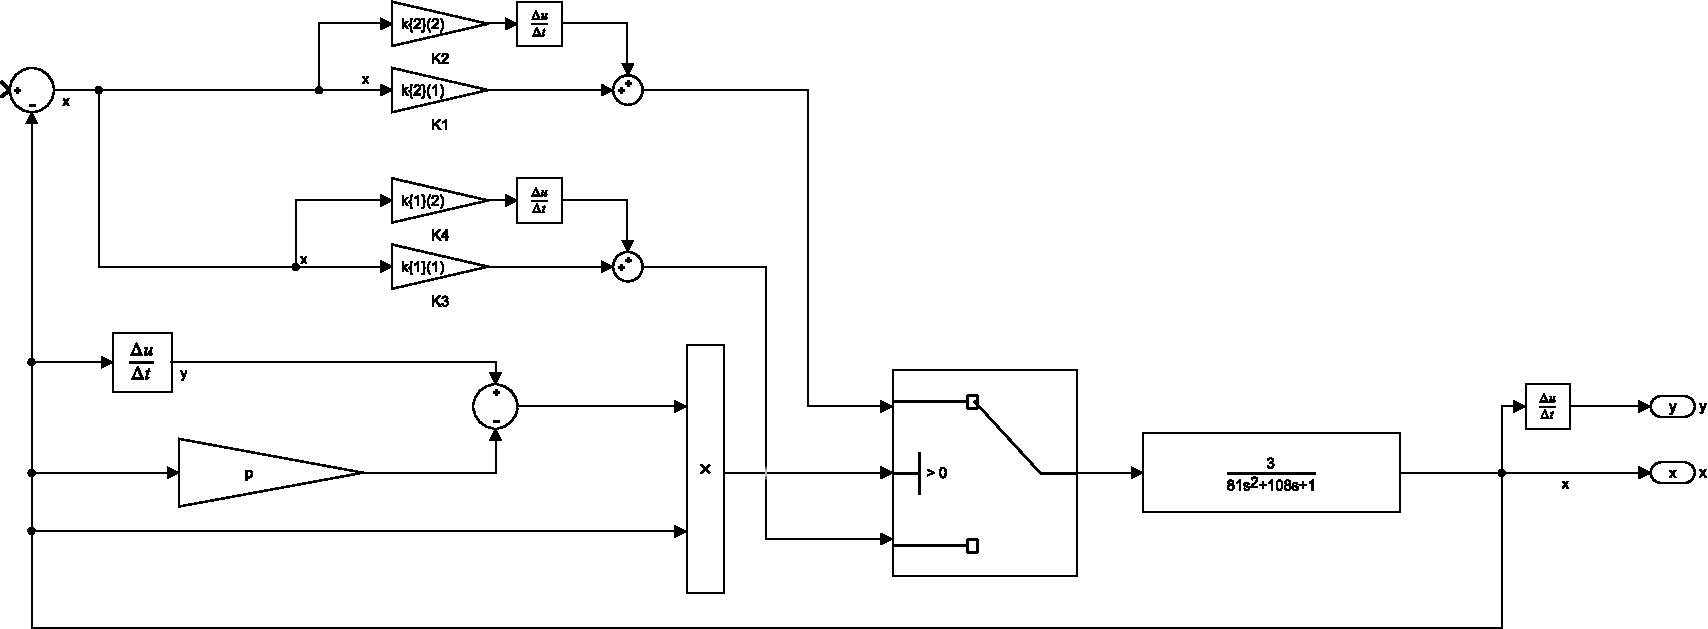
\includegraphics[width=1.0\linewidth]{images/sim_VSS_steady_degenerate_motion}
\caption{Структурная схема системы с переменной структурой с вырожденным устойчивым движением}\label{fig:sim_VSS_steady_degenerate_motion}
\end{figure}
Исследуем движение фазовых координат во времени посредством моделирования процессов в системе при отклонении системы от состояния равновесия. Фазовые траектории в системе на рис.\ref{fig:VSS_steady_degenerate_motion_ft_SDM}. 
В дополнение на рис.\ref{fig:VSS_steady_degenerate_motion_sv_SDM} указано изменение выходной переменной и её производной. 
\begin{figure}[!h]\centering
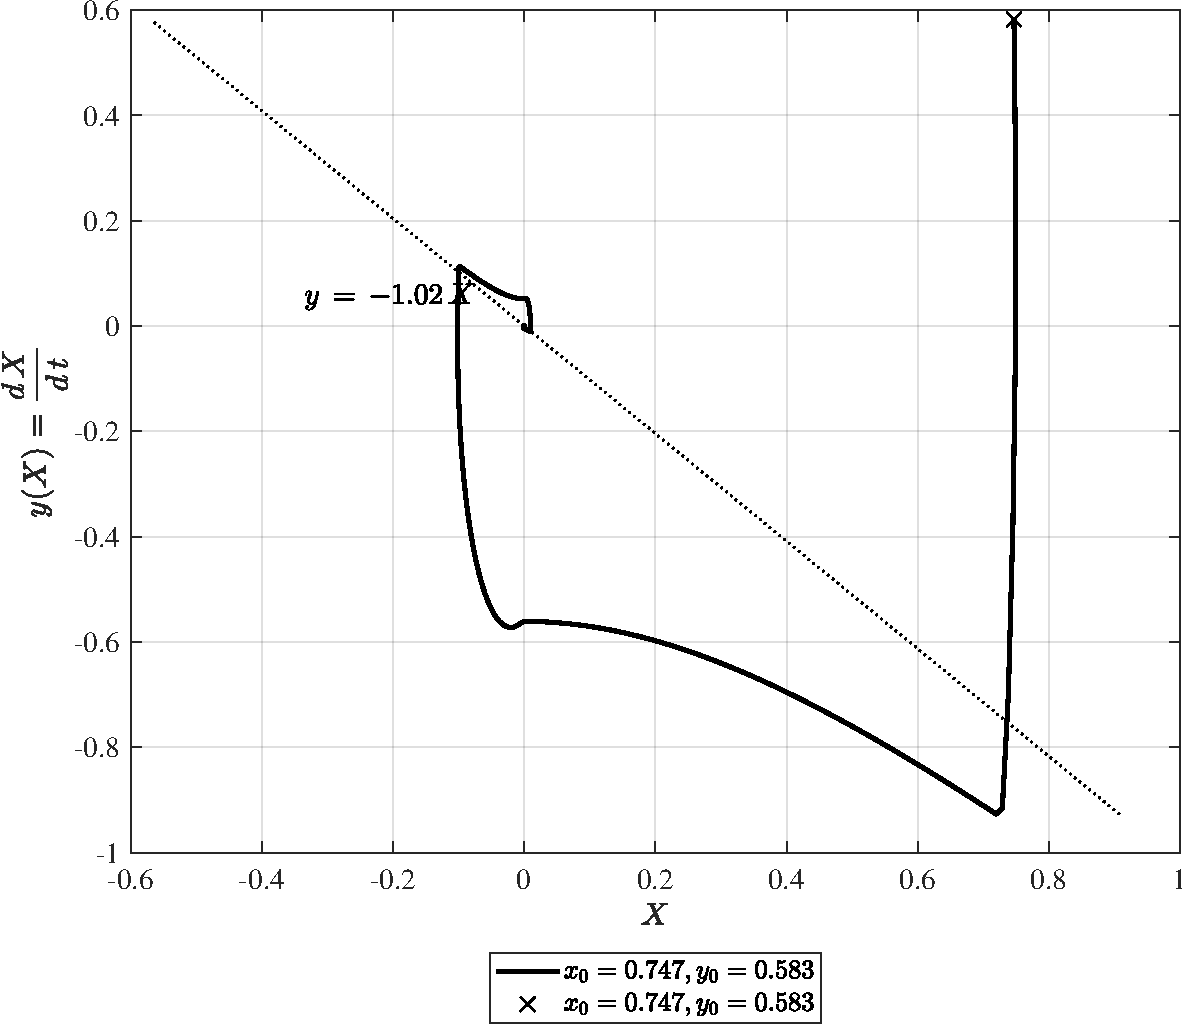
\includegraphics[width=1.0\linewidth]{images/VSS_steady_degenerate_motion_ft_SDM}
\caption{ Фазовые траектории для системы с переменной структурой с разными начальными условиями.}\label{fig:VSS_steady_degenerate_motion_ft_SDM}
\end{figure}
\begin{figure}[!h]\centering
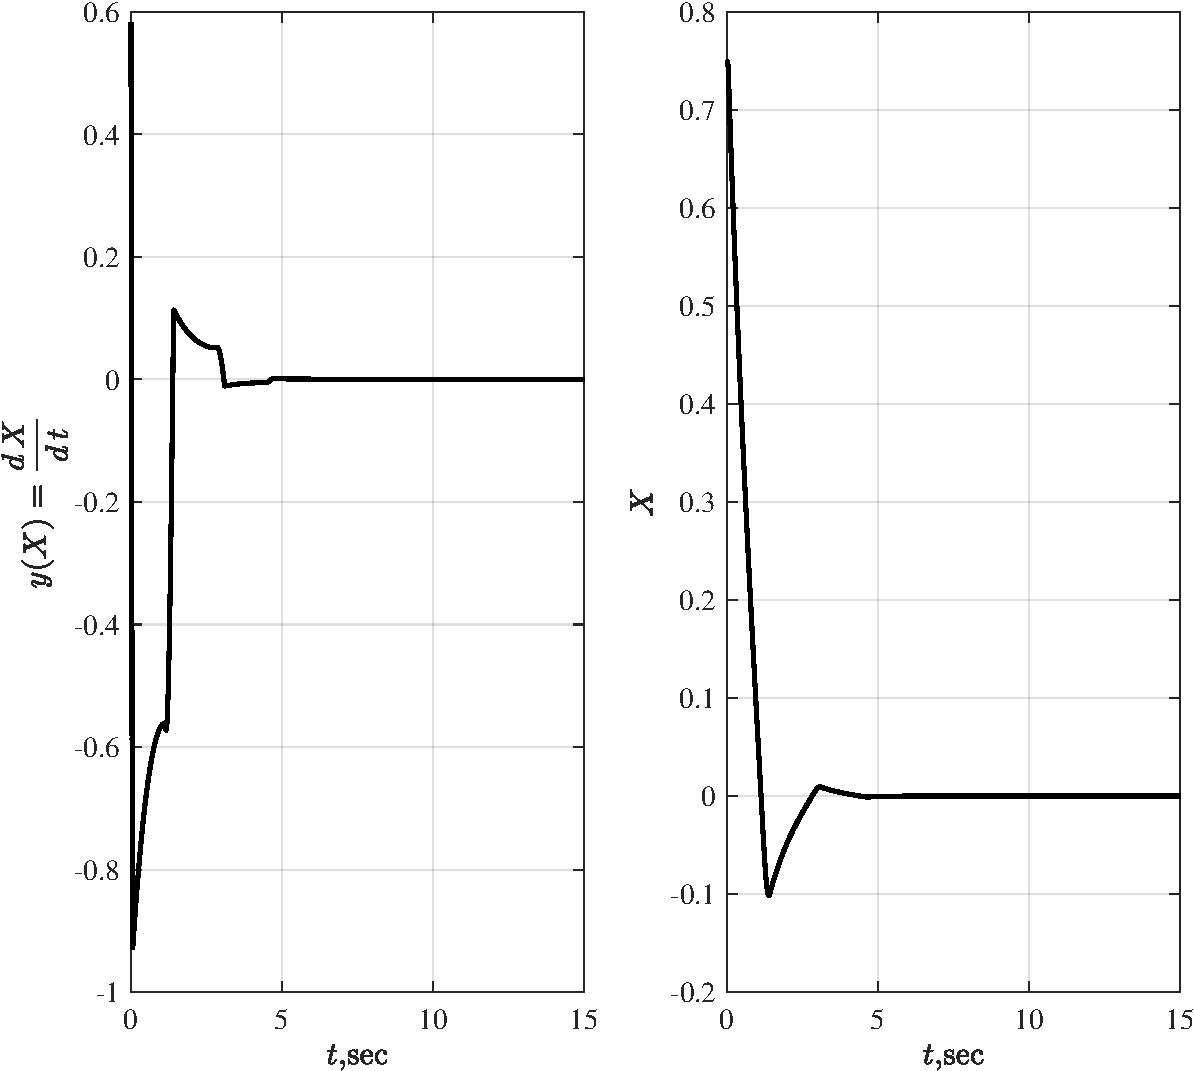
\includegraphics[width=1.0\linewidth]{images/VSS_steady_degenerate_motion_sv_SDM}
\caption{ Графики изменения выходной переменной и её производной.}\label{fig:VSS_steady_degenerate_motion_sv_SDM}
\end{figure}

Этот подход позволяет построить устойчивую систему и отказаться от требований устойчивости для каждой из имеющихся структур. Однако в рассматриваемом случае движение по линии переключения отсутствует, так как инерционные силы смещают изображающую точку с этой линии, её дальнейшее движение происходит по другой фазовой траектории, но в целом движение остаётся асимптотически устойчивым - фазовая траектория стягивается к началу координат. 
